%%%%%%%%%%%%%%%%%%%%%%%%%%%%%%%%%%%%%%%%%%%%%%%%%%%%%%%%%%%%%%%%%%%%%%%%%%
\chapter{Analýza bajtkódu}\label{Analysis}

% Popis způsobu analýzy rozsáhlého vzorku testovacích dat, prezentace výsledků a zhodnocení.

V~této kapitole popisuji analýzu bajtkódu a její výsledky. Pomocí nástroje \texttt{jbyco} jsem získala data reprezentující velký vzorek testovacích souborů a tato data následně analyzovala a vyhodnotila. Zkoumala jsem velikosti položek v~\texttt{class} souborech, využití lokálních proměnných a parametrů a typické sekvence bajtkódu.

Testovací vzorek jsem vytvořila z~\texttt{jar} souborů stažených z~\texttt{http://mvnrepository.com}. Z~populárních kategorií jsem vybrala nejčastěji používané \texttt{jar} soubory. Po smazání příliš velkých souborů jsem získala testovací vzorek o~velikosti 92 souborů a 102,4 MB. Pro analýzu typických sekvencí jsem musela zvolit menší vzorek o~velikosti 6 souborů a 1,1 MB, neboť pro více dat mi nestačila paměť.

\section{Výsledky analýzy}\label{AnalysisResults}

Využití parametrů a lokálních proměnných je znázorněné na grafech \ref{params} a \ref{vars}. Zajímalo mne, kolikrát se z~daného parametru či lokální proměnné načítá hodnota a vkládá hodnota. Počet operací je zprůměrován celkovým počtem výskytů daného parametru či lokální proměnné. Z~grafu \ref{params} lze vyčíst, že z~parametrů se především načítají hodnoty ale už se do nich nic neukládá. Jejich celkové využití je velmi malé. S~lokálními proměnnými se pracuje častěji, ale jejich využití mohlo být pořád lepší.

\begin{figure}[h!]
\centering
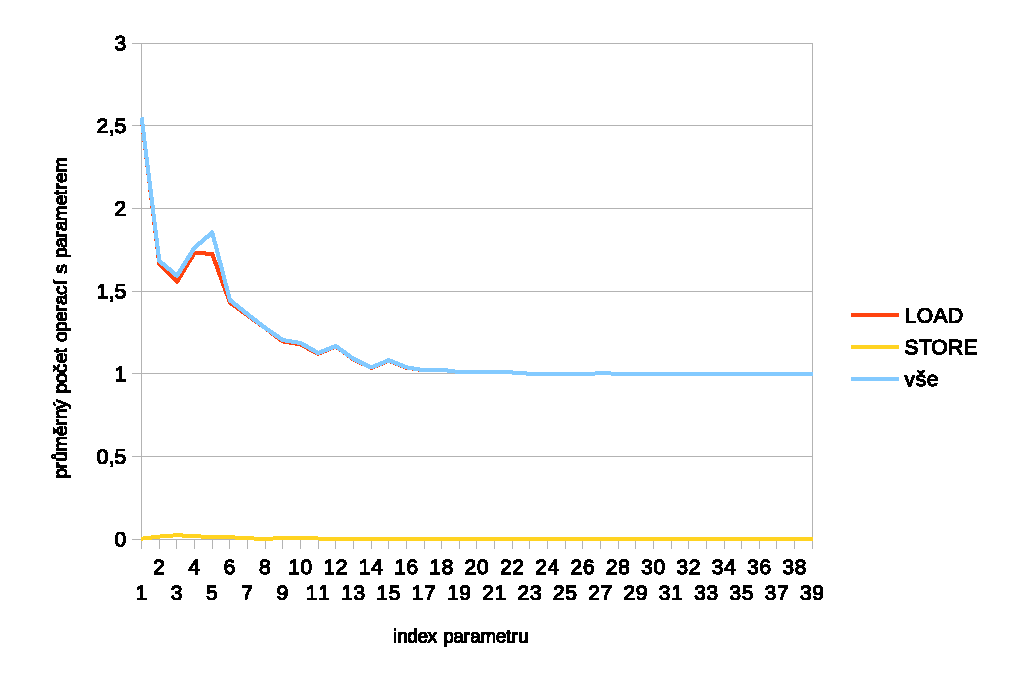
\includegraphics[scale=0.9]{fig/params}
\caption{Průměrné počty operací s~danými parametry.}\label{params}
\end{figure}

\begin{figure}[h!]
\centering
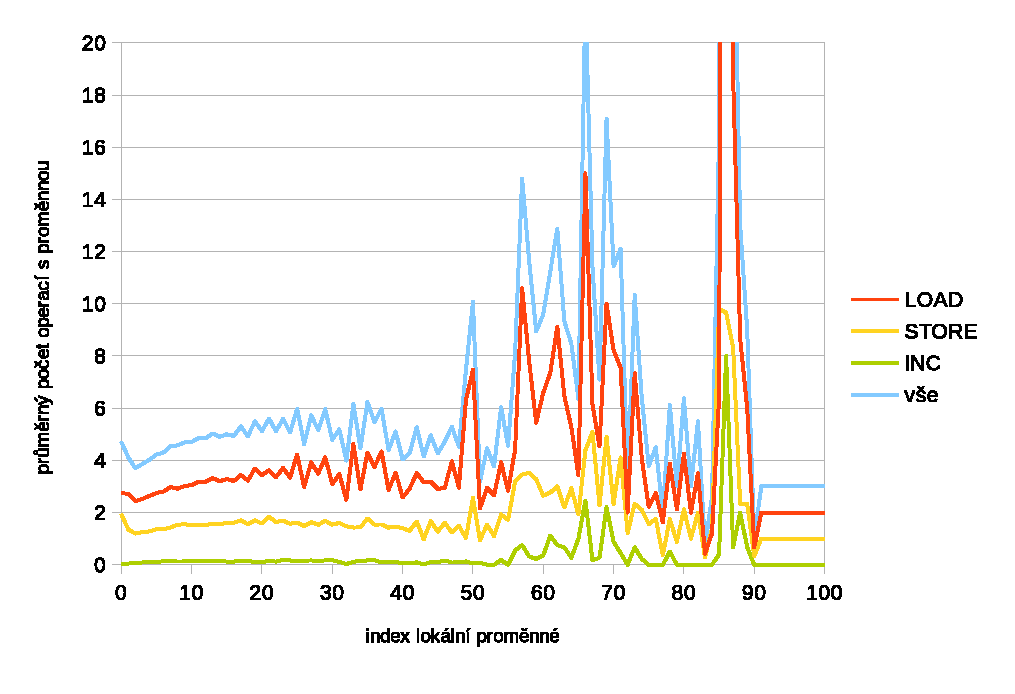
\includegraphics[scale=0.9]{fig/locals} 
\caption{Průměrné počty operací s~danými lokálními proměnnými.}\label{vars}
\end{figure}


Při analýze velikosti jsem zkoumala konstanty, atributy a instrukce z~hlediska celkového počtu a celkové velikosti. Z~tabulek \ref{constf} a \ref{consts} je zřejmé, že konstanta \texttt{CONSTANT\_Utf8} je nejfrekventovanější a zároveň zabírá ze všech konstant největší procento z~celkové velikosti souboru. Následují konstanty pro popis metod, tříd, rozhraní a členských proměnných. A~poslední v~pořadí jsou číselné konstanty.
Nejfrekventovanějším a nejobjemnějším atributem je podle tabulek \ref{attrf} a \ref{attrs} pochopitelně \texttt{Code}. Zajímavé však je, že velké procento atributů i celkové velikosti tvoří atributy sloužící výhradně pro ladící účely.
V~tabulkách \ref{instf} a \ref{insts} jsou zjištěné hodnoty pro instrukce. Prvenství v~četnosti instrukce \texttt{aload\_0} lze vysvětlit častým používáním reference \texttt{this}. Následují instrukce pro volání metody a načtení hodnoty z~proměnné instance. Podle dalších konstant v~tabulce je zřejmé, že se nejčastěji pracuje s~referencí na objekt.
Z~hlediska celkové velikosti jsou nejobjemnější instrukce pro volání metod a získávání hodnoty členské proměnné.

Přehled typických sekvencí operačních kódů je dostupný v~tabulce \ref{seq}. Nejčastější sekvence \texttt{aload\_0;getfield;} poukazuje na častý přístup k~proměnným aktuální instance. Sekvence \texttt{new;dup;} reprezentuje optimalizaci. Dále se často pracuje s~prvními dvěma lokálními proměnnými. Nejčastěji se spolu v~jedné sekvenci objevuje načítání reference z~lokální proměnné a volání speciálních metod.

\section{Vyhodnocení}\label{AnalysisSummary}

Studium využití parametrů a lokálních proměnných poukazuje na plýtvání s~tímto paměťovým prostorem. Pole lokálních proměnných by zřejmě mohlo být menší, kdyby se proměnné více recyklovaly. Použití parametrů jako lokálních proměnných zase umožní používat instrukce s~kratšími kódy.

Z~analýzy velikosti konstant plyne, že řetězce tvoří podstatnou část instrukčního souboru. Řetězcové konstanty a řetězce s~typy nijak nahradit nelze, ale názvy tříd, rozhraní, metod a proměnných by bylo možné nahradit kratšími řetězci. 
Analýza velikosti atributů poukázala na to, že atributy, které nemají vliv na interpretaci souboru, mají poměrně velkou velikost. Tyto atributy by za jistých předpokladů šlo odstranit.
Z~analýzy velikosti instrukcí vyplynulo, že se nejčastěji používají objemné instrukce. To stejné se potvrdilo analýzou typických sekvencí. Bylo by vhodné se zamyslet nad tím, jak zamezit zbytečnému volání metod a načítání hodnot z~členských proměnných. 



% Shrnutí výsledků a komentář. Jak mohu výsledky analýzy použít pro další postup práce?

%=========================================================================
